%#Split: 02_purpose_plan  
%#PieceName: p02_purpose_plan
% p02_purpose_plan_00.tex
\KLBeginSubjectWithHeaderCommands{02}{}{研究目的・内容等}{2}{F}{}{\DCPDFirstSubjectPageStyle}{\DCPDDefaultPageStyle}

\section{研究目的・内容等}
%    <<最大 2ページ>>

%s02_purpose_plan_dcpd
%begin 研究目的と研究計画short留意事項なし ====================
%begin 研究計画における研究目的、研究方法、研究内容 ====================
\graysubsection{①研究計画における研究目的、研究方法、研究内容}
\vspace{20pt}
\sbsbsection{研究目的}
本研究では、フェイクニュースの早期自動検出を日本語で実現するために、
データセットの作成から検出モデルの実装を目的とする。
さらに、実装したモデルの汎化性能向上に向けて改善を続ける。

\sbsbsection{研究方法・研究内容}

\setlength\intextsep{0pt}
\setlength\textfloatsep{0pt}
\begin{wrapfigure}{r}[0pt]{0.6\linewidth}
    \vspace{-5mm}
    \centering
    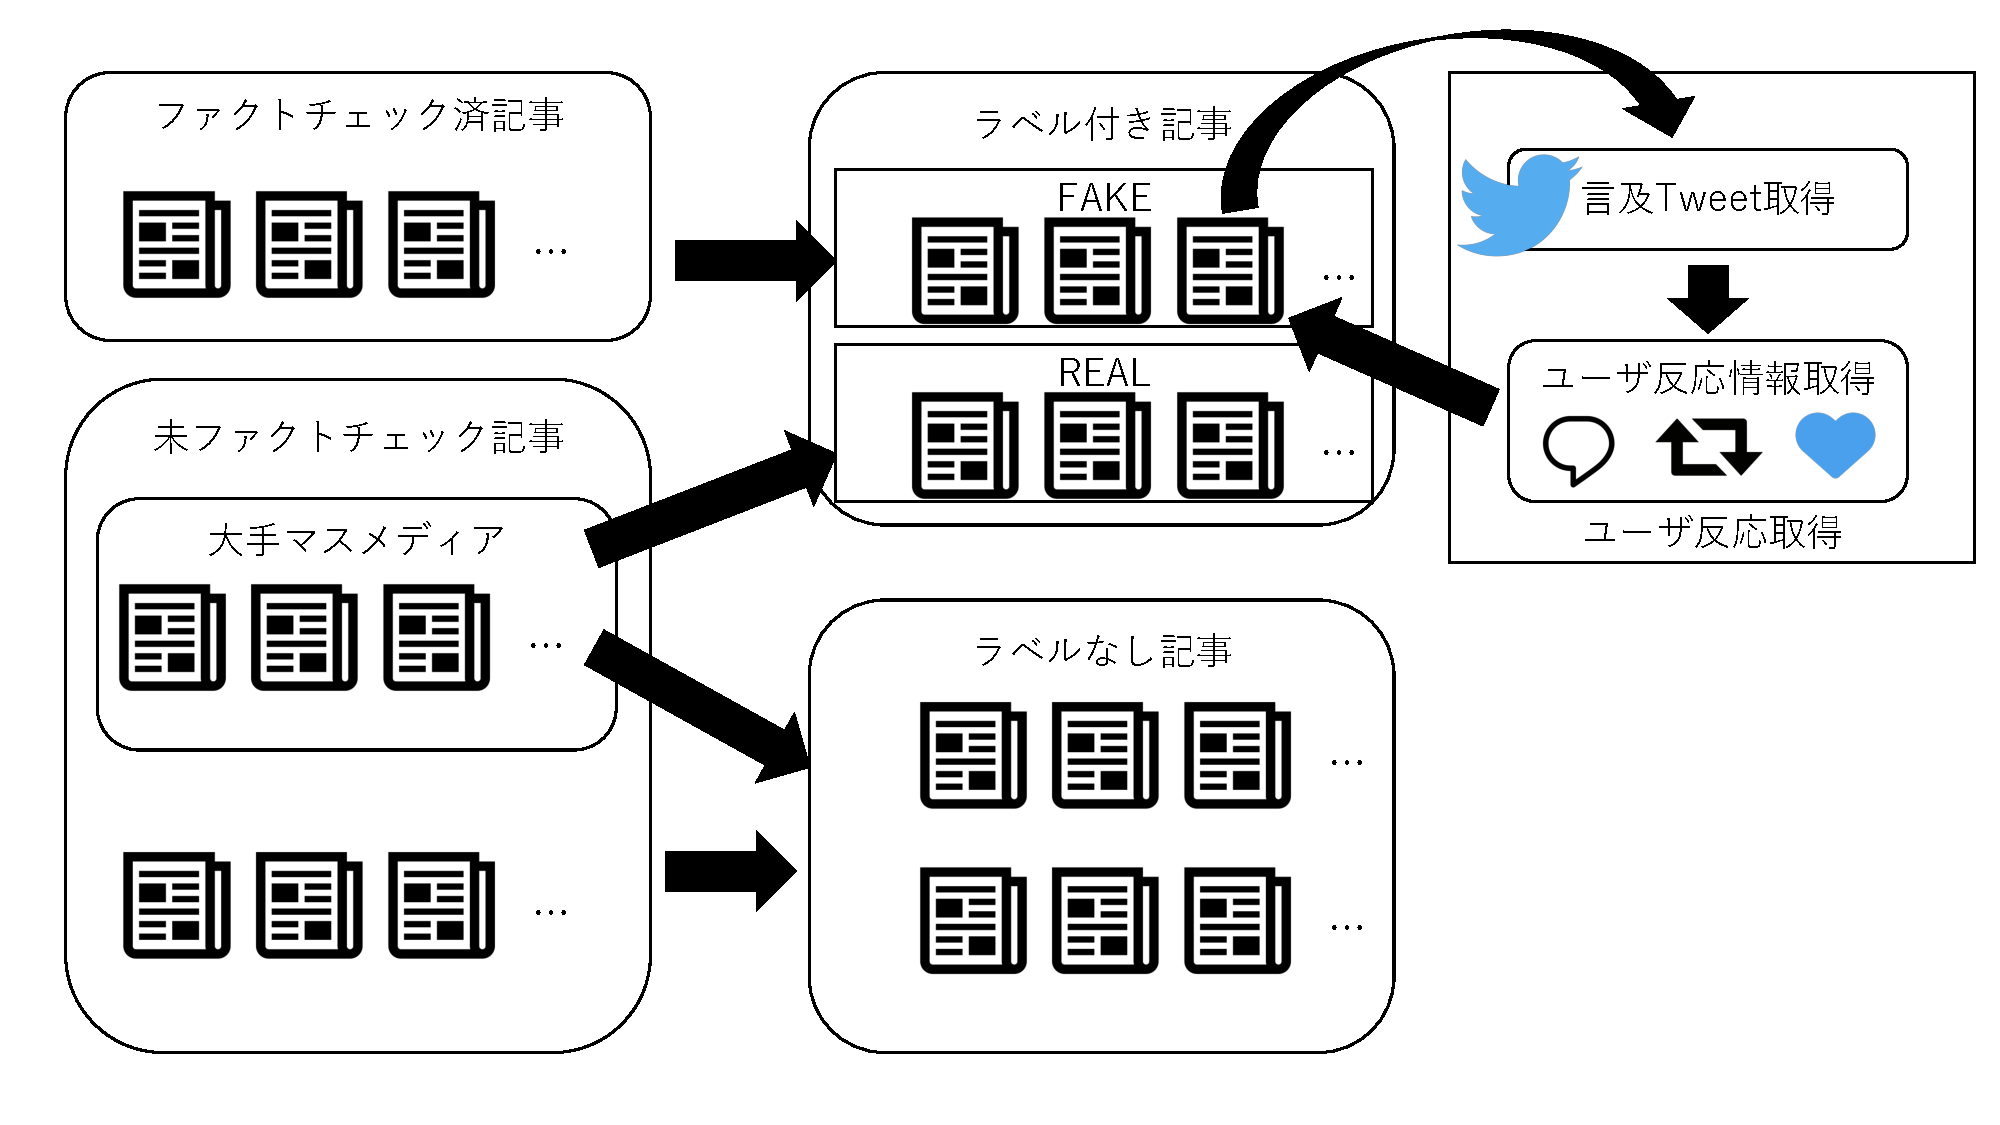
\includegraphics[width=0.6\textwidth]{figs/dataset.pdf}
    \vspace{-1cm} 
    \caption{データセット作成の流れ。ユーザ反応取得は全記事を対象に行う。}
    \label{fig:dataset}
\end{wrapfigure}

以下の3目標を目指し研究する。
\begin{description}
    \item[目標Ⅰ] データセット作成に向けファクトチェック済記事とそうでない記事、同時にSNS上で記事に寄せられたコメントやユーザ情報等を収集する。
    \item[目標Ⅱ] 早期検出を想定した状況で高精度な真偽分類を行うモデルをユーザの初期反応から得られた弱いアノテーションと共に行う。
    \item[目標Ⅲ] 汎化性能向上に向けて内製以外のデータセットを用いても性能が劣化しないようモデルの改変を行う。
\end{description}

%end 研究計画における研究目的、研究方法、研究内容 ====================

%begin どのような計画で、何を、どこまで明らかにしようとするのか ====================
\graysubsection{②どのような計画で、何を、どこまで明らかにしようとするのか}
\vspace{20pt}
\sbsbsection{目標Ⅰ: 日本語の記事・真偽を含むデータセットを作成する(採用前 - 1年目)}
日本語での検出を実現するためには、まずはデータセットを作成する必要がある。
データセット作成の全体の流れは図\ref{fig:dataset}の通りである。
%完全教師あり学習・弱教師あり学習に問わず最低限必要なものは記事情報とファクトチェック結果による真偽ラベルである。
日本語ファクトチェック結果の取得には、特定非営利活動法人ファクトチェック・イニシアティブ(以下FIJ)が提供するFactCheck Naviを使用する。
2021年4月現在で600超件のファクトチェック結果が公表されている。%おり、FIJが提供するガイドライン\cite{fij}に基づき9種類のレーティングが行われている。
%今回はその中で``誤り''、``虚偽''、``ミスリード''、``不正確''、``根拠不明''と評価された記事をフェイクと扱う。
一方ファクトチェックにより正確と判断された事例はフェイクに比べて少な%く、2021年4月中旬現在FactCheck Naviの直近20件のファクトチェック結果は全てフェイクに該当する。
いため、正確なニュースとして大手新聞社やロイター通信等の記事を収集する。

また目標Ⅱに向けて正解ラベルがなく、弱いアノテーションを付加する対象である記事を追加する。
正確とみられるニュースは先述と同じく大手マスメディアが発信したニュースを扱い、
疑わしい記事としてFactCheck Naviによって虚偽と3回以上判断されたことがあるニュースサイトの他記事も収集対象とする。
最終的には真偽合わせて\underline{ラベル付き記事を約1200件}、\underline{ラベルなし記事を約5000件以上}収集を目指す。
ユーザの反応として、全記事を対象にSNS上で寄せられたコメントとしてTwitterにて記事URLを含むツイートも収集する。

\sbsbsection{目標Ⅱ: 弱教師あり学習によってラベル不足を補うモデルを構築する(1年目)}
\setlength\intextsep{0pt}
\setlength\textfloatsep{0pt}
\begin{wrapfigure}{r}[0pt]{0.8\linewidth}
    \vspace{-5mm}
    \centering
    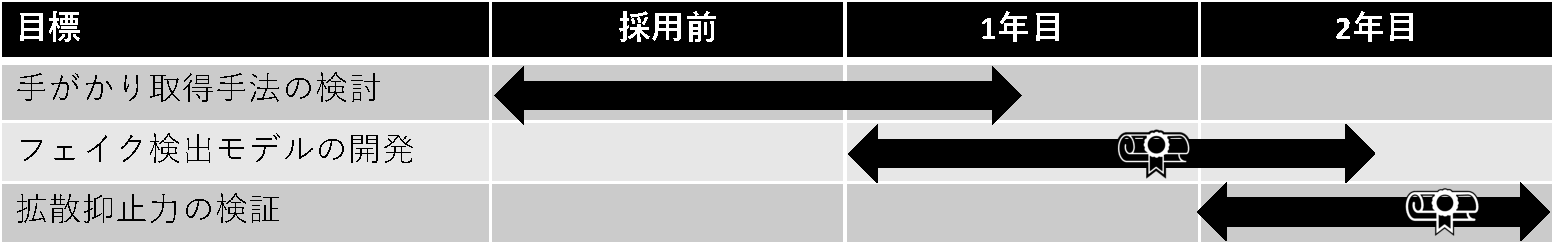
\includegraphics[width=0.8\textwidth]{figs/plan.pdf}
    \vspace{-1cm} 
    \caption{研究計画の年毎の流れ。}
    \label{fig:plan}
\end{wrapfigure}
ラベル付きユーザの反応を弱いアノテーションとして扱ってフェイクニュースを検出する方法は、
英文記事を対象にしたKai Shuらの研究で1例が示されている\cite{shu2020leveraging}。
ここではコメント群の感情値の標準偏差やコメント者の過去の投稿、そしてフォロー関係から弱いアノテーションを付加している。
これら3種の弱いアノテーションも併せて学習することで、\underline{推論時はユーザの反応を使わずに正確な早期検出を実現}した。
今回はこの3種類に加え、他に投稿者のプロフィールや使用された絵文字やハッシュタグといった情報で有用なものがないか模索する。

\sbsbsection{目標Ⅲ: トピックに左右されない汎化性能向上を模索する(2年目)}
更に提案手法の汎化性能を向上させるため、\underline{別のデータセットでも有用か}調べる。
日本語データセットは数が乏しいため、複数バリエーションがある英語で実験を行う予定である。
候補としては先行研究で既に頻繁に採用されているFakeNewsNet\cite{fakenewsnet}というファクトチェック済英文記事などを予定している。

実験では学習と推論を同じデータセット内で完結させた時と別のデータセットで行った時を比較させ、
目標は2値(真・偽)分類時の総合指標であるF値や正解率の差が10パーセントポイント以下とする。

%end どのような計画で、何を、どこまで明らかにしようとするのか ====================

%begin 研究の特色・独創的な点 ====================
\graysubsection{③研究の特色・独創的な点}
\vspace{20pt}
\sbsbsection{本研究の特色}
\begin{itemize}
    \item \underline{日本語}を対象にフェイクニュースの自動検出を行う点。
    \item ファクトチェックの結果を待たず\underline{早期の検出}を目指す点。
    \item 変化する社会情勢を踏まえ、\underline{特定の記事カテゴリに限らず高精度な検出}を行う点。
\end{itemize}

\sbsbsection{先行研究との比較}
深層学習でフェイクニュースを自動検出する\underline{研究対象は英文に集中}しており、
\underline{日本語データセットがない}。
言語に囚われずユーザによる拡散された経緯で真偽を判断する研究もあるが\cite{tarek2020}、
依然として記事の内容を考慮した研究では日本語を対象としたものがない。

\sbsbsection{予想されるインパクト・将来の見通し}
総務省によるとSNS利用率は2019年現在69\%を占める上、SNSマーケティング市場規模は2025年に1兆1,171億円まで成長する(出典:サイバー・バズ/デジタルインファクト調べ)と推測されている。
SNS利用者が拡大を続ける中、本研究の完成によりこれまで活発になされていなかった日本語のフェイクニュースを早期検出するモデルの開発および提供が可能となる。
SNS利用者への注意喚起に活用ができるほか、ファクトチェックを行う人への補助システムへの活用
といった様々な形式でSNS上で騙される人が増え社会的損害や風評被害の発生を未然に防ぐ枠組み作りに貢献する可能性がある。

%end 研究の特色・独創的な点 ====================

%begin 申請者が担当する部分 ====================
\graysubsection{④申請者が担当する部分}
本研究は所属研究室内でも萌芽的な取り組みで、環境・技術面の支援を除き\underline{申請者が全部分を担当}する。
データセットの生成では、正確なニュースの取得へ大手マスメディアへ協力を求める可能性がある。
%end 申請者が担当する部分 ====================

%begin 受入研究機関と異なる研究機関での研究従事計画 ====================
\graysubsection{⑤受入研究機関と異なる研究機関での研究従事計画}
申請者は\underline{1年間タリン工科大学の言語技術研究所(Tanel Alumäe所長)で活動予定}である。
当該分野は北米と欧州の研究が活発であることから、\underline{最前線の研究に従事}するために必要である。
%end 受入研究機関と異なる研究機関での研究従事計画 ====================

\vspace{1cm}
{\footnotesize 
\begin{twobibliography}{99}
    \setlength{\parskip}{0cm}
    \setlength{\itemsep}{0cm}
    %\bibitem{fij} FIJ. 2019: ファクトチェック・ガイドライン
    \bibitem{shu2020leveraging} Kai S., \textit{et al.} \textit{ECML-PKDD 2020}
    \bibitem{fakenewsnet} Kai S,\textit{et al.} \textit{Big Data 8.3} 2020: 171-188.
    \bibitem{tarek2020} Tarek H., \textit{et al.} \textit{ICDCIT 2020}
\end{twobibliography}
}
%end 研究目的と研究計画short留意事項なし ====================
% p02_purpose_plan_01.tex
\KLEndSubject{F}


